%% Compile with
%% Rscript -e "library(knitr); knit('test-knitr.Rnw')" &
%% pdflatex test.tex

\documentclass{article}\usepackage[]{graphicx}\usepackage[]{color}
% maxwidth is the original width if it is less than linewidth
% otherwise use linewidth (to make sure the graphics do not exceed the margin)
\makeatletter
\def\maxwidth{ %
  \ifdim\Gin@nat@width>\linewidth
    \linewidth
  \else
    \Gin@nat@width
  \fi
}
\makeatother

\definecolor{fgcolor}{rgb}{0.345, 0.345, 0.345}
\newcommand{\hlnum}[1]{\textcolor[rgb]{0.686,0.059,0.569}{#1}}%
\newcommand{\hlstr}[1]{\textcolor[rgb]{0.192,0.494,0.8}{#1}}%
\newcommand{\hlcom}[1]{\textcolor[rgb]{0.678,0.584,0.686}{\textit{#1}}}%
\newcommand{\hlopt}[1]{\textcolor[rgb]{0,0,0}{#1}}%
\newcommand{\hlstd}[1]{\textcolor[rgb]{0.345,0.345,0.345}{#1}}%
\newcommand{\hlkwa}[1]{\textcolor[rgb]{0.161,0.373,0.58}{\textbf{#1}}}%
\newcommand{\hlkwb}[1]{\textcolor[rgb]{0.69,0.353,0.396}{#1}}%
\newcommand{\hlkwc}[1]{\textcolor[rgb]{0.333,0.667,0.333}{#1}}%
\newcommand{\hlkwd}[1]{\textcolor[rgb]{0.737,0.353,0.396}{\textbf{#1}}}%
\let\hlipl\hlkwb

\usepackage{framed}
\makeatletter
\newenvironment{kframe}{%
 \def\at@end@of@kframe{}%
 \ifinner\ifhmode%
  \def\at@end@of@kframe{\end{minipage}}%
  \begin{minipage}{\columnwidth}%
 \fi\fi%
 \def\FrameCommand##1{\hskip\@totalleftmargin \hskip-\fboxsep
 \colorbox{shadecolor}{##1}\hskip-\fboxsep
     % There is no \\@totalrightmargin, so:
     \hskip-\linewidth \hskip-\@totalleftmargin \hskip\columnwidth}%
 \MakeFramed {\advance\hsize-\width
   \@totalleftmargin\z@ \linewidth\hsize
   \@setminipage}}%
 {\par\unskip\endMakeFramed%
 \at@end@of@kframe}
\makeatother

\definecolor{shadecolor}{rgb}{.97, .97, .97}
\definecolor{messagecolor}{rgb}{0, 0, 0}
\definecolor{warningcolor}{rgb}{1, 0, 1}
\definecolor{errorcolor}{rgb}{1, 0, 0}
\newenvironment{knitrout}{}{} % an empty environment to be redefined in TeX

\usepackage{alltt}
\usepackage[T1]{fontenc}
\usepackage{url}
\usepackage[unicode=true,pdfusetitle]{hyperref}
\IfFileExists{upquote.sty}{\usepackage{upquote}}{}
\begin{document}


\title{My knitr demo}
\author{Michael Ash}
\maketitle

You can test if \textbf{knitr} works with this minimal demo. OK, let's
get started with some boring random numbers:

\begin{knitrout}
\definecolor{shadecolor}{rgb}{0.969, 0.969, 0.969}\color{fgcolor}\begin{kframe}
\begin{alltt}
\hlkwd{set.seed}\hlstd{(}\hlnum{1121}\hlstd{)}
\hlstd{(x}\hlkwb{=}\hlkwd{rnorm}\hlstd{(}\hlnum{20}\hlstd{))}
\end{alltt}
\begin{verbatim}
##  [1]  0.1449583  0.4383221  0.1531912  1.0849426  1.9995449
##  [6] -0.8118832  0.1602680  0.5858923  0.3600880 -0.0253084
## [11]  0.1508809  0.1100824  1.3596812 -0.3269946 -0.7163819
## [16]  1.8097690  0.5084011 -0.5274603  0.1327188 -0.1559430
\end{verbatim}
\begin{alltt}
\hlstd{(xbar}  \hlkwb{<-} \hlkwd{mean}\hlstd{(x)); (xvar}  \hlkwb{<-} \hlkwd{var}\hlstd{(x))}
\end{alltt}
\begin{verbatim}
## [1] 0.3217385
## [1] 0.5714534
\end{verbatim}
\end{kframe}
\end{knitrout}

The first element $X_1$ of \texttt{x} is 0.1449583. Rounded to two decimal places, the mean is 0.32 and the variance is 0.57.

Here are the annotated results of a couple of coin tosses (at this
point we hand random-number generation back to the system:
\begin{knitrout}
\definecolor{shadecolor}{rgb}{0.969, 0.969, 0.969}\color{fgcolor}\begin{kframe}
\begin{alltt}
\hlkwd{set.seed}\hlstd{(}\hlkwd{Sys.time}\hlstd{())}
\end{alltt}
\end{kframe}
\end{knitrout}



The coin comes up heads.



Here is the result of another coin toss.  The coin comes up tails instead.

A boring plot in ggplot can be see in Figure~\ref{fig:boring}.

\begin{figure}
  \caption{A boring figure}
  \label{fig:boring}
\begin{knitrout}
\definecolor{shadecolor}{rgb}{0.969, 0.969, 0.969}\color{fgcolor}

{\centering 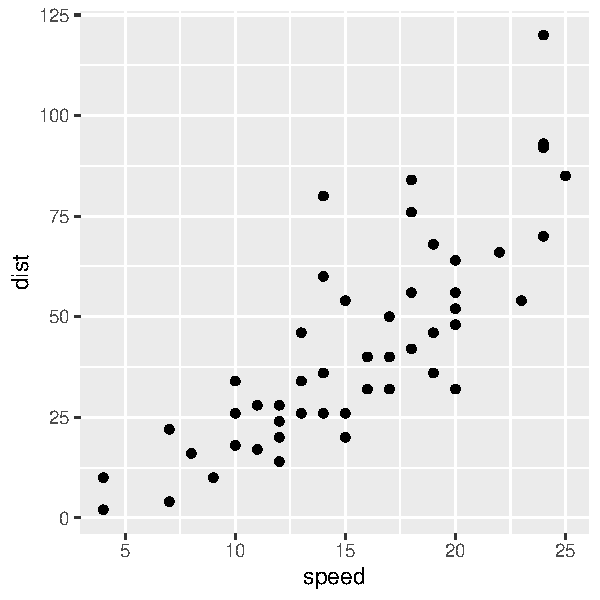
\includegraphics[width=.6\linewidth]{figure/minimal-boring-plots-1} 

}


\end{knitrout}
\end{figure}

Summary statistics are in Table~\ref{tab:summary}.

\begin{kframe}
\begin{alltt}
\hlkwd{stargazer}\hlstd{(cars,} \hlkwc{title}\hlstd{=}\hlstr{"Summary statistics"}\hlstd{,} \hlkwc{label}\hlstd{=}\hlstr{"tab:summary"}\hlstd{)}
\end{alltt}
\end{kframe}
% Table created by stargazer v.5.2.2 by Marek Hlavac, Harvard University. E-mail: hlavac at fas.harvard.edu
% Date and time: Tue, Nov 16, 2021 - 12:31:24 PM
\begin{table}[!htbp] \centering 
  \caption{Summary statistics} 
  \label{tab:summary} 
\begin{tabular}{@{\extracolsep{5pt}}lccccccc} 
\\[-1.8ex]\hline 
\hline \\[-1.8ex] 
Statistic & \multicolumn{1}{c}{N} & \multicolumn{1}{c}{Mean} & \multicolumn{1}{c}{St. Dev.} & \multicolumn{1}{c}{Min} & \multicolumn{1}{c}{Pctl(25)} & \multicolumn{1}{c}{Pctl(75)} & \multicolumn{1}{c}{Max} \\ 
\hline \\[-1.8ex] 
speed & 50 & 15.400 & 5.288 & 4 & 12 & 19 & 25 \\ 
dist & 50 & 42.980 & 25.769 & 2 & 26 & 56 & 120 \\ 
\hline \\[-1.8ex] 
\end{tabular} 
\end{table} 


And the regression results are in Table~\ref{tab:regression}




\begin{kframe}
\begin{alltt}
\hlkwd{stargazer}\hlstd{(model1, model2, model3,} \hlkwc{title}\hlstd{=}\hlstr{"Regression results"}\hlstd{,} \hlkwc{label}\hlstd{=}\hlstr{"tab:regression"}\hlstd{)}
\end{alltt}
\end{kframe}
% Table created by stargazer v.5.2.2 by Marek Hlavac, Harvard University. E-mail: hlavac at fas.harvard.edu
% Date and time: Tue, Nov 16, 2021 - 12:31:24 PM
\begin{table}[!htbp] \centering 
  \caption{Regression results} 
  \label{tab:regression} 
\begin{tabular}{@{\extracolsep{5pt}}lccc} 
\\[-1.8ex]\hline 
\hline \\[-1.8ex] 
 & \multicolumn{3}{c}{\textit{Dependent variable:}} \\ 
\cline{2-4} 
\\[-1.8ex] & \multicolumn{3}{c}{dist} \\ 
\\[-1.8ex] & (1) & (2) & (3)\\ 
\hline \\[-1.8ex] 
 speed & 3.932$^{***}$ & 0.913 & 6.801 \\ 
  & (0.416) & (2.034) & (6.801) \\ 
  & & & \\ 
 I(speed$\hat{\mkern6mu}$2) &  & 0.100 & $-$0.350 \\ 
  &  & (0.066) & (0.500) \\ 
  & & & \\ 
 I(speed$\hat{\mkern6mu}$3) &  &  & 0.010 \\ 
  &  &  & (0.011) \\ 
  & & & \\ 
 Constant & $-$17.579$^{**}$ & 2.470 & $-$19.505 \\ 
  & (6.758) & (14.817) & (28.405) \\ 
  & & & \\ 
\hline \\[-1.8ex] 
Observations & 50 & 50 & 50 \\ 
R$^{2}$ & 0.651 & 0.667 & 0.673 \\ 
Adjusted R$^{2}$ & 0.644 & 0.653 & 0.652 \\ 
Residual Std. Error & 15.380 (df = 48) & 15.176 (df = 47) & 15.205 (df = 46) \\ 
F Statistic & 89.567$^{***}$ (df = 1; 48) & 47.141$^{***}$ (df = 2; 47) & 31.584$^{***}$ (df = 3; 46) \\ 
\hline 
\hline \\[-1.8ex] 
\textit{Note:}  & \multicolumn{3}{r}{$^{*}$p$<$0.1; $^{**}$p$<$0.05; $^{***}$p$<$0.01} \\ 
\end{tabular} 
\end{table} 




\begin{kframe}
\begin{alltt}
\hlkwd{stargazer}\hlstd{(model1, model2, model3,} \hlkwc{title}\hlstd{=}\hlstr{"Regression results with new names"}\hlstd{,} \hlkwc{label}\hlstd{=}\hlstr{"tab:regression:newnames"}\hlstd{)}
\end{alltt}
\end{kframe}
% Table created by stargazer v.5.2.2 by Marek Hlavac, Harvard University. E-mail: hlavac at fas.harvard.edu
% Date and time: Tue, Nov 16, 2021 - 12:31:24 PM
\begin{table}[!htbp] \centering 
  \caption{Regression results with new names} 
  \label{tab:regression:newnames} 
\begin{tabular}{@{\extracolsep{5pt}}lccc} 
\\[-1.8ex]\hline 
\hline \\[-1.8ex] 
 & \multicolumn{3}{c}{\textit{Dependent variable:}} \\ 
\cline{2-4} 
\\[-1.8ex] & \multicolumn{3}{c}{dist} \\ 
\\[-1.8ex] & (1) & (2) & (3)\\ 
\hline \\[-1.8ex] 
 speed & 3.932$^{***}$ & 0.913 & 6.801 \\ 
  & (0.416) & (2.034) & (6.801) \\ 
  & & & \\ 
 Speed-squared &  & 0.100 & $-$0.350 \\ 
  &  & (0.066) & (0.500) \\ 
  & & & \\ 
 Speed-cubed &  &  & 0.010 \\ 
  &  &  & (0.011) \\ 
  & & & \\ 
 Constant & $-$17.579$^{**}$ & 2.470 & $-$19.505 \\ 
  & (6.758) & (14.817) & (28.405) \\ 
  & & & \\ 
\hline \\[-1.8ex] 
Observations & 50 & 50 & 50 \\ 
R$^{2}$ & 0.651 & 0.667 & 0.673 \\ 
Adjusted R$^{2}$ & 0.644 & 0.653 & 0.652 \\ 
Residual Std. Error & 15.380 (df = 48) & 15.176 (df = 47) & 15.205 (df = 46) \\ 
F Statistic & 89.567$^{***}$ (df = 1; 48) & 47.141$^{***}$ (df = 2; 47) & 31.584$^{***}$ (df = 3; 46) \\ 
\hline 
\hline \\[-1.8ex] 
\textit{Note:}  & \multicolumn{3}{r}{$^{*}$p$<$0.1; $^{**}$p$<$0.05; $^{***}$p$<$0.01} \\ 
\end{tabular} 
\end{table} 



Do the chunks work? You should be able to compile the \LaTeX{} document.




\end{document}



